\documentclass[twocolumn, 11pt]{article}%
\usepackage{amsmath, amssymb, esint, gensymb, hyperref, mathtools}
\usepackage{graphicx, cuted, geometry, float, scalerel, xcolor, xfrac}

\newcommand\sbullet[1][.5]{\mathbin{\ThisStyle{\vcenter{\hbox{%
  \scalebox{#1}{$\SavedStyle\bullet$}}}}}%
}

\geometry{
    a4paper,
    total={170mm,260mm},
}

\begin{document}

\begin{strip}
  \vspace*{\dimexpr-\stripsep}
  \begin{center}
      \Large\textbf{FISIKA 2}\\
      \large{Pertemuan 2 - Minggu 9 (475017)}\\
      \large{\today}
   \end{center}
\end{strip}

\section{Perhitungan Medan Magnet}
\subsection{Induksi Magnet Oleh Arus Listrik}%

\begin{center}
    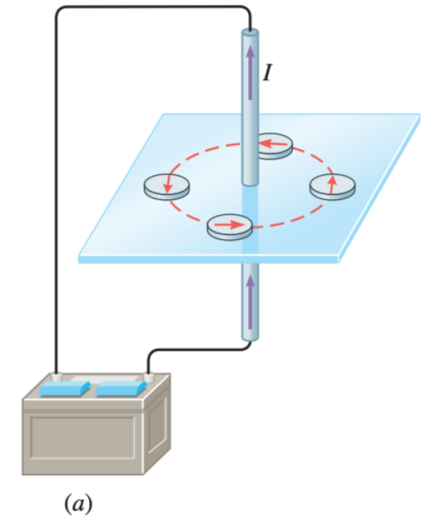
\includegraphics[width=100px]{1.png}
    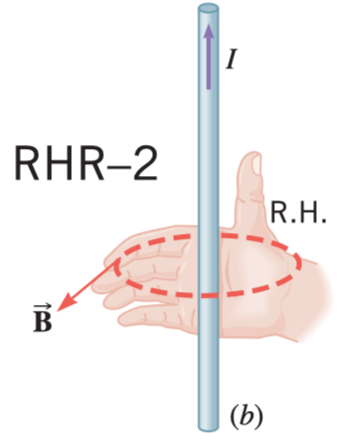
\includegraphics[width=100px]{2.png}
\end{center}
Hans Christian $\O$rsted melakukan pengamatan pertama kali pada kawat
lurus yang sangat panjang yang dialiri arus listrik dan menemukan bahwa
Kompas yang berada di dekat kabel tersebut akan berubah arahnya sesuai
dengan aturan tangan kanan.

Untuk lebih lengkapnya silahkan mengunjungi \url{https://www.youtube.com/watch?v=RwilgsQ9xaM}

\subsection{Perhitungan Medan Magnet}%
\subsubsection{Elemen dari Kawat}%

\begin{center}
    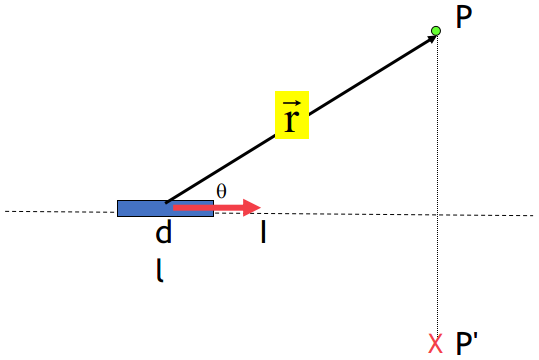
\includegraphics[width=150px]{3.png}
\end{center}

Sebelumnya diketahui bahwa:\\
\begin{itemize}
    \item $\vec R$ adalah vektor dari $dl$ ke \textbf{P}.
    \item $\displaystyle k'=\frac{\mu_0}{4\pi}=10^{-7} \text{ Wb/A.m}$
    \item Permeabilitas\\
          $\mu_0=12,57.10^{-7} \text{ Wb/A.m}$
\end{itemize}

Lalu Medan Magnet di titik P pada jarak \textbf{r} dari elemen arus
\textbf{I dl} :

\[d\vec B = \frac{\mu_0}{4\pi} \frac{I\
\overrightarrow{dI}\times \vec r}{r^3} \]

atau
\[dB = \frac{k'\ I\ dL\sin \theta}{r^2} \]

Selanjutnya rumus diatas disebut dengan Hukum Biot-Savart.

\subsubsection{Kawat Lurus}%
\begin{center}
    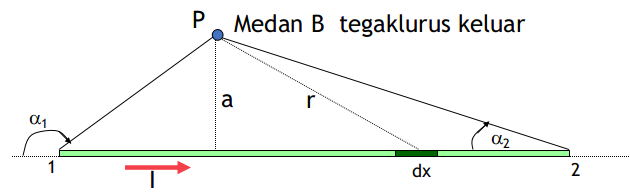
\includegraphics[width=200px]{4.png}
    Bisa dibayangkan arah medan magnetnya \textbf{Tegak Lurus keluar
    Bidang Kertas}.
    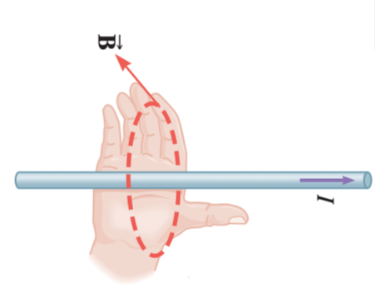
\includegraphics[width=110px]{5.png}
\end{center}

Lalu, besar medan magnet B adalah
\[B=\frac{k'I}{a}(\cos \alpha_2 - \cos \alpha_1)\]

Bila kawat sangat panjang, $\infty$. Maka
\begin{itemize}
    \item $\alpha_2 =0\degree$
    \item $\alpha_1 =180\degree$
\end{itemize}

Sehingga
\[B=\frac{\mu_0 I}{2\pi a} \]

\subsubsection{Gaya Pada Dua Kawat Berarus Sejajar}%
\begin{center}
    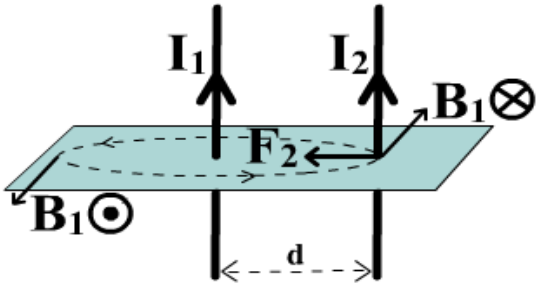
\includegraphics[width=160px]{6.png}
\end{center}

Pada kasus semacam ini, Medan magnet yang ditimbulkan oleh arus $I_1$
pada jarak $d$ adalah
\[B_1=\frac{\mu_0 I_1}{2\pi d} \]

Sementara itu Arus $I_2$ berada dalam medan $B_1$, maka $I_2$ mengalami gaya
\[ F_{21} = I_2 L_2 B_1 \]

Gaya per satuan panjang pada kawat berarus $I_2$ adalah
\[\frac{F_{21}}{L_2} =\frac{\mu_0 I_1I_2}{2\pi d} \]

Arahnya bisa dilihat pada gambar di atas.

\subsubsection{Kawat Lingkaran}%
\begin{center}
    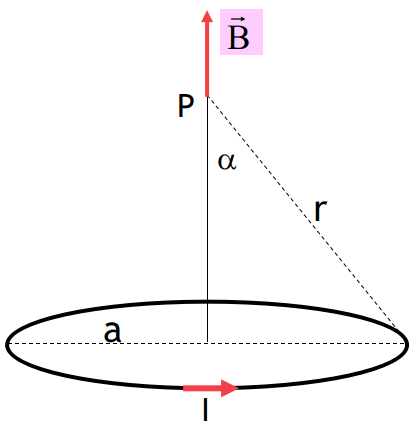
\includegraphics[width=100px]{7.png}
    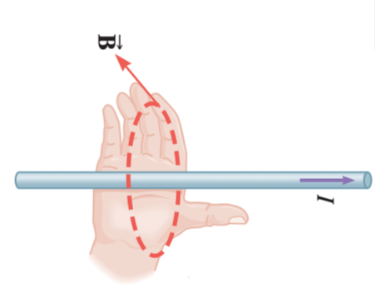
\includegraphics[width=110px]{5.png}
\end{center}

Di titik P, besar medan magnet B adalah
\[B=\frac{k'\ I \sin \alpha}{r^2}. 2\pi a \]

Bila terdapat N lilitan
\[B=N.\frac{k'\ I \sin \alpha}{r^2}. 2\pi a \]

Bila titik P di pusat lingkaran, $\alpha = 90\degree$. Sehingga
\[B=\frac{\mu_0 I}{2a} \]

Bila terdapat N lilitan
\[B=\frac{\mu_0 NI}{2a} \]

\subsubsection{Busur Lingkaran}%
\begin{center}
    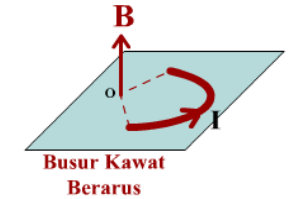
\includegraphics[width=150px]{8.png}
\end{center}

\[B=\frac{\mu_0}{4\pi}.\frac{I}{a^2}.S \]

dengan
\begin{itemize}
    \item a = jari – jari busur lingkaran.
    \item S = panjang busur.
\end{itemize}

\subsubsection{Selenoida}%
\begin{center}
    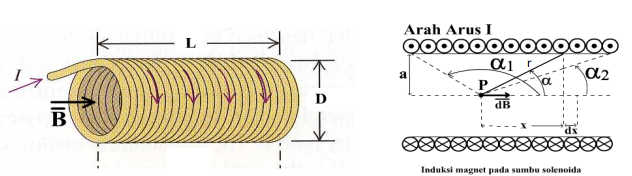
\includegraphics[width=220px]{9.png}
\end{center}

Sehingga medan magnet pada selenoida adalah
\[B=\frac{\mu_0 NI}{2L}(\cos \alpha_2 - \cos \alpha_1) \]

Dimana N adalah jumlah lilitan pada selenoida. Pada kasus di mana
selenoida sangat panjang, $a<<L$, maka
\begin{itemize}
    \item $\alpha_2 = 0\degree$
    \item $\alpha_1 = 180\degree$
\end{itemize}

Sehingga
\[B=\frac{\mu_0 NI}{L} \]

\subsubsection{Toroida}%
\begin{center}
    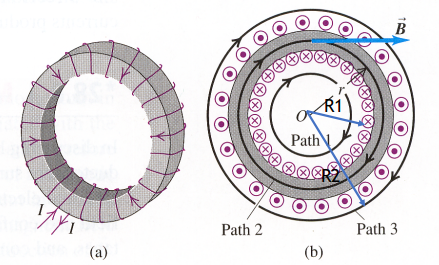
\includegraphics[width=200px]{10.png}
\end{center}

dengan
\begin{itemize}
    \item Jari-jari dalam adalah $\mathbf{R_1}$
    \item Jari-jari luar adalah $\mathbf{R_2}$
\end{itemize}


\[B=\frac{\mu_0 NI}{L} = \frac{\mu_0 NI}{\pi(R_1+R_2)} \]

Hal ini dikarenakan
\begin{itemize}
    \item $L=2\pi r$
    \item $\displaystyle r=\frac12 (R_1+R_2)$
\end{itemize}

\subsection{Fluks Magnetik $\Phi$}%
Pada definisinya, fluks magnetik ($\Phi$) adalah jumlah garis induksi
magnetik yang menembus sebuah permukaan tertentu.

\begin{center}
    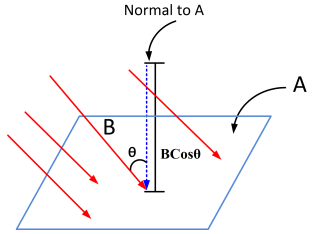
\includegraphics[width=150px]{11.png}
\end{center}

\[\Phi=BA\cos\theta \]

Satuan fluks magnetik ($\Phi$) adalah \textbf{Weber} atau \textbf{Tesla
$\mathbf{m^2}$}.\\

Pada kasus dimana $\theta=0\degree$, maka
\[\Phi=BA \]

Perhatikan gambar berikut,
\begin{center}
    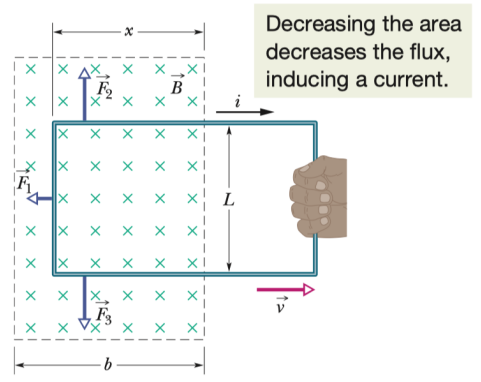
\includegraphics[width=150px]{12.png}
\end{center}

Jadi diketahui bahwa
\[A=L.x\]


\end{document}
